\documentclass[10pt, physics]{homework}

\usepackage{geometry}
\usepackage{graphicx}

\title{Assignment 1}
\course{ASTR 356b}
\due{6 February 2018}
\author{Jackson Petty}

\newcommand\floor[1]{\left\lfloor #1 \right\rfloor}
\newcommand\ceiling[1]{\left\lceil #1 \right\rceil}

\begin{document}
	\begin{problem}[4pts]
		Consider two urns. The first contains two white and seven black balls, and the second contains five white and six black balls. We flip a fair coin and then draw a ball from the first or the second urn depending on whether the outcome was heads or tails. What is the conditional probability that the outcome of the toss was heads given that a white ball was selected?
	\end{problem}
	\begin{proof}[Solution]
		Let $P(W)$ denote the probability that the coin flip results in a heads (implying that the ball is chosen from Urn 1), and $P(U)$ denote the probability that a white ball is drawn.
		By the law of total probability, we know that 
		\[ P(W) = P(W \cap \text{Urn 1}) + P(W \cap \text{Urn 2}). \]
		Since the coin is fair, we know that the total probability of drawing a white ball is then
		\[ P(W) = \frac{1}{2}\qty[\frac{2}{9} + \frac{5}{11}] = \frac{67}{198}. \]
		Then by Bayes's theorem, we calculate that the probability that the ball was chosen from Urn 1, given that it was white, is
		\[ P(H \mid W) = \frac{P(W \mid H) \cdot P(H)}{P(W)} = \frac{(2/9) \cdot (1/2)}{67/138} = \final{\frac{22}{67} \approx 32.84\%.}\qedhere \]
	\end{proof}

	\begin{problem}[4pts]
		A laboratory blood test is 95\% effective in detecting a certain disease when it is, in fact, present. However, the test yields a ``false positive'' result for 1\% of healthy persons tested (i.e., probability = 0.01 for healthy person to test positive on test). If 0.5\% of population has disease, what is the probability that a person has the disease given that his/her test results is positive.
	\end{problem}
	\begin{proof}[Solution]
		Let $P(D)$ denote the probability that one has the blood disease, and $P(T)$ be the probability that the test results for the disease are positive.
		By the law of total probability, we know that 
		\[ P(T) = P(T \cap \text{Has Disease}) + P(T \cap \text{False Positive}), \]
		which, by the given values, would mean that 
		\[ P(T) = \frac{19}{20}\frac{1}{200} + \frac{1}{100}\frac{199}{200} = \frac{147}{10\,000}. \]
		Using Bayes' theorem, we see then that the probability that the one has the disease given a positive result is 
		\[ P(D \mid T) = \frac{P(T \mid D)\cdot P(D)}{P(T)} = \frac{(19/20)\cdot(1/200)}{147/10\,000} = \final{\frac{95}{294} \approx 32.31\%.}\qedhere \]
	\end{proof}

	\begin{problem}[4pts]
		Let us suppose that we count a large number of quasars in many different parts of the sky to obtain an average surface density of quasars, per square degree. An astronomer is investigating quasar counts in one area of sky and finds an unusually large number of quasars, $N_0$, in the area of one square degree. Does this indicate anisotropy or is it a random fluctuation? The probability of finding exactly $N$ quasars is given by the Poisson distribution. 
		\begin{parts}
			\part[part:3:a] Assume that the mean is $2$ and that $N_0 = 5$. What is the probability of finding $N \geq N_0$ quasars?
			\part[part:3:b] The astronomer searched through 20 such fields before finding the result quoted above ($N=5$). Do you think the astronomer can claim that the universe is anisotropic? Why or why not?
		\end{parts}
	\end{problem}
	\begin{proof}[Solution to~\ref{part:3:a}]
		If the probability of finding $N$ quasars is modeled by a Poisson distribution, then we know that
		\[ P(N = n) = \frac{\lambda^n \e^{-\lambda}}{n!}, \]
		where $n$ is the number of quasars observed and $\lambda = 2$ is the number of quasars expected.
		If we want to find $P(N \geq N_0)$, we use the CDF
		\[ F_n({N_0-1}) = \e^{-\lambda} \sum_{i=0}^{\lfloor N_0 \rfloor} \frac{\lambda^i}{i!}, \]
		which gives us the probability of finding less that $N_0$ quasars, and then subtract that value from unity.
		In our case, we see that 
		\[ F_n(4) = \e^{-2}\sum_{i = 0}^4 \frac{2^i}{i!} = \frac{7}{e^2}. \]
		Then $P(N \geq N_0) = 1 - F_n(4) \approx \final{5.2653\%.}$
	\end{proof}
	\begin{proof}[Solution to~\ref{part:3:b}]
		If the astronomer searched through 20 fields before encountering one with $N = 5$ quasars, then it seems like the probability of finding such a field due to random fluctuation is on the order of $1/20 \approx 5\%$.
		Since the probability of finding a field with more than $N_0$ quasars as modeled by a Poisson distribution is $5.2653\%$, it seems likely that this was due to random fluctuation, not anisotropy.
	\end{proof}

	\begin{problem}[4pts]
		In a quasar survey covering an area of 1000 square degrees on the sky, the total number of quasars found is 2340. Assuming that the projected distribution of quasars can be modeled as a Poisson distribution, what is the probability of observing less than 5 quasars in a given square degree of the sky? What area of sky could one expect to survey before the probability of finding no quasars was less than 1\%?
	\end{problem}
	\begin{proof}[Solution]
		If 2340 quasars were found in 1000 square degrees of sky, then the expected number of quasars $\lambda = 2.34$.
		As before, we model the probability of finding less than $N_0 + 1$ quasars using the Cumulative Distibution Function for a Poisson distribution, given by
		\[ F_n(N_0 + 1) = \e^{-\lambda} \sum_{i = 0}^{\floor{N_0}} \frac{\lambda^i}{i!}. \]
		In our case, we have $N_0 = 4$ (since the CDF gives us the probability of finding $P(X \leq N_0)$, and we want the probability of finding \emph{less} than 5 quasars, not \emph{at most} 5 quasars), so the probability is
		\[ F_n(5) = \e^{-2.34} \sum_{i=0}^4 \frac{2.34^i}{i!} \approx \final{91.1504\%.} \]
		The probability of finding \emph{no} quasars is given by 
		\[ F_n(1) = \e^{-2.34} \approx 9.6328\% \text{ per square degree.} \]
		We then need to find an $m$ such that $\qty[F_n(1)]^m < 0.01$, which is found simply by
		\[ m = \ceiling{\log_{0.096328}(0.01)} = \final{2 \text{ square degrees.}} \qedhere \]
	\end{proof}

	\begin{problem}[10pts]
		An astronomer has a sample of optically selected active galactic nuclei (AGN, such as Seyfert galaxies and quasi-stellar objects or QSOs) and surveys them with a radio telescope to estimate the fraction of AGN that produce non-thermal radio emission from a relativistic jet. Let $X$ denote the random variable giving the result of the radio-loudness test, where $X = 1$ indicates a positive and $X = 0$ indicates a negative result. Let $\theta_1$ denote that radio-loudness is present and $\theta_2$ that the AGN is radio-quiet. $P(\theta = \theta_1)$ denotes the probability that a randomly chosen AGN is radio-loud (this is the prevalence of radio-loudness in the optically-selected AGN population). From previous surveys the astronomer expects the prevalence is 0.1, but this is not based on the observational data under study. Based on the known sensitivity of the radio telescope and the AGN redshift distribution, the astronomer can establish that the radio survey is sufficiently sensitive to measure the radio emission 80\% of the time in radio-loud AGN (the failures are due to AGN at very high redshifts). However, the sample also includes some AGN at small redshifts where the telescope may detect other kind of radio emission (e.g., from star formation in the host galaxy). This occurs 30\% of the time. What is the probability that an AGN is truly radio-loud when a positive detection is obtained, $P(\theta  = \theta_1 \mid X = 1)$? Show with a plot how the probability $P(\theta = \theta_1 \mid X = 1)$ changes as the probability of obtaining a false positive decreases from 30\%  to 5\%.
	\end{problem}
	\begin{proof}[Solution]
		We know by the law of total probability that 
		\[ P(X = 1) = \frac{4}{5}\frac{1}{10} + \frac{3}{10}\frac{9}{10} = \frac{7}{20}. \]
		We then use Bayes' theorem to determine that the probability that an AGN is loud given a positive detection is 
		\[ P(\theta = \theta_1 \mid X = 1) = \frac{P(X = 1 \mid \theta = \theta_1)\cdot P(\theta = \theta_1)}{P(X = 1)} = \frac{(4/5)\cdot(1/10)}{7/20} = \final{\frac{8}{35} \approx 22.86\%.}\qedhere \]
		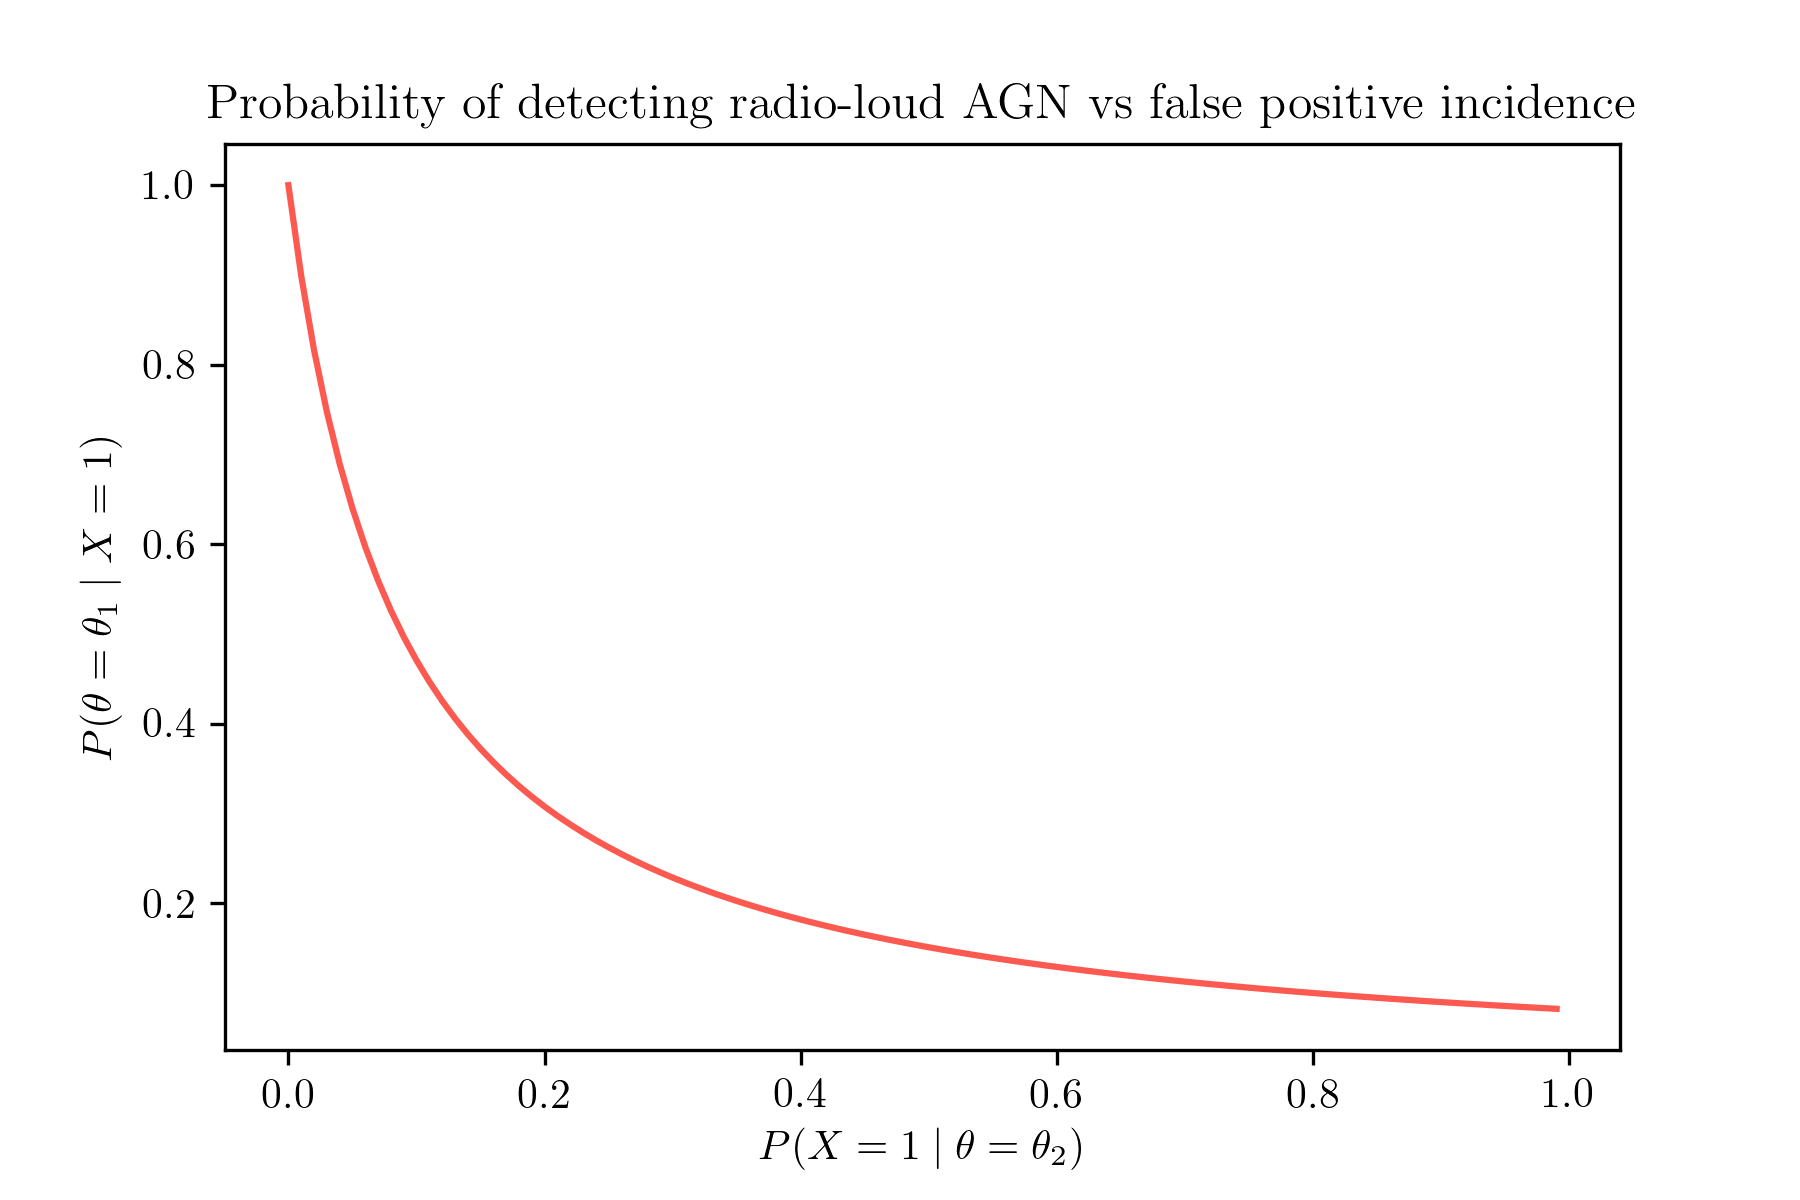
\includegraphics{plot}

	\end{proof}

	\begin{problem}[12pts]
		The probability density function $f(x)$ of a hypothetical measurement is given by the triangular function shown below (Figure 1), where the value of $f(0)$ is called $C$. 
		\begin{parts}
			\part[part:6:a] Find $C$ in terms of $a$.
			\part[part:6:b] What are the mean and variance of $f(x)$? Do this both analytically and numerically.
			\part[part:6:c] What is the probability of a measurement with $x > 0$? Do this both analytically and numerically.
			\part[part:6:d] Sketch this function for the cases that $a = 1$ and $a =2$.
		\end{parts}
	\end{problem}
	\begin{proof}[Solution to~\ref{part:6:a}]
		We know that integrating over the whole distribution must give unity, so we see that 
		\[ \frac{1}{2}(a - (-a))\cdot C = 1 \implies C = \final{\frac{1}{a}.}\qedhere \]
	\end{proof}
	\begin{proof}[Solution to~\ref{part:6:b}]
		The variance of $f(x)$ is given analytically by
		\[ \text{Var}\qty(f(x)) = \frac{(-a)^2 + (a) + c^2 - (a)(-a) - a(0) - (-a)(0)}{18} = \final{\frac{a^2}{6}.} \]
		The mean of $f(x)$ is given analytically by 
		\[ \text{Mean}\qty(f(x)) = \frac{(-a) + a + 0}{3} = \final{0.}\qedhere \]
	\end{proof}
	\begin{proof}[Solution to~\ref{part:6:c}]
		Using the CDF for a symmetric triangular distribution, we see that 
		\[ P(X \leq x) = \frac{(x-a)^2}{(b-a)(b-c)} = \frac{a^2}{2a^2} = \final{\frac{1}{2}.}\qedhere \]
	\end{proof}

	\begin{problem}[12pts]
		The Monty Hall problem is a well-known problem in statistics based on a game show. The scenario is that a contestant is given a choice of 3 doors. Behind one of them is the grand prize, while the other 2 doors have goats. (Obviously, you don’t want to have a goat.) After the contestant decides for a door, hoping to have chosen the winner, the game show master opens one of the doors. The show master knows what is behind each door, so he will never open the door with the prize and he also does not open the contestant’s door. After opening the door, the show master asks the contestant whether he wants to switch his door to the other remaining one. The question is: Should the contestant change his choice. In other words, would that increase his chances of winning? Perform computer simulations to answer that question. Does that answer make sense? Write down an analytical derivation, as well.
	\end{problem}
\end{document}